\chapter*{Введение}                         % Заголовок
\addcontentsline{toc}{chapter}{Введение}    % Добавляем его в оглавление

\newcommand{\actuality}{}
\newcommand{\progress}{}
\newcommand{\aim}{{\textbf\aimTXT}}
\newcommand{\tasks}{\textbf{\tasksTXT}}
\newcommand{\novelty}{\textbf{\noveltyTXT}}
\newcommand{\influence}{\textbf{\influenceTXT}}
\newcommand{\methods}{\textbf{\methodsTXT}}
\newcommand{\defpositions}{\textbf{\defpositionsTXT}}
\newcommand{\reliability}{\textbf{\reliabilityTXT}}
\newcommand{\probation}{\textbf{\probationTXT}}
\newcommand{\contribution}{\textbf{\contributionTXT}}
\newcommand{\publications}{\textbf{\publicationsTXT}}

{\actuality} Магнитоэлектрические эффекты обусловлены наличием в термодинамическом потенциале членов, линейных как по электрическому, так и по магнитному полю \autocite{Landau}. Данные эффекты наблюдаются в магнитоэлектриках и мультиферроиках в случае, когда одновременно нарушается симметрия относительно обращения знака времени (следствие магнитного упорядочения) и симметрия относительно пространственной инверсии (особенности кристаллической структуры) - магнитными свойствами этих материалов можно управлять прикладывая внешнее электрическое поле и наоборот. Так, авторы работы \autocite{Saito2008ape} наблюдали в антиферромагнетике \cbo\ вращение намагниченности, индуцированное электрическим полем. Позднее другая группа смогла управлять электрической поляризацией \ncbo\ с помощью внешнего магнитного поля \autocite{Khanh2013}. Кроме указанных \emph{статических} магнитоэлектрических эффектов наблюдаются также \emph{динамические} - обусловленные взаимодействием с периодическими электромагнитными полями. В частности, к таковым относятся явление невзаимности (nonreciprocity) в спектрах поглощения \autocite{Toyoda2015} и явление пространственной асимметрии люминесценции (directional asymmetry of luminescence) \autocite{Toyoda2016}.  

Интерес к этим эффектам в последние десятилетия существенно возрос, в связи с реальными перспективами практических применений. На основе магнитоэлектрических материалов можно создавать магнитные запоминающие устройства с оптическим считыванием информации о доменной структуре, управляемые магнитным полем оптические диоды и пр. Выяснение микроскопической природы (механизмов) этих эффектов важно для фундаментальных научных знаний.

\begin{figure}[ht]
	\centerfloat{
		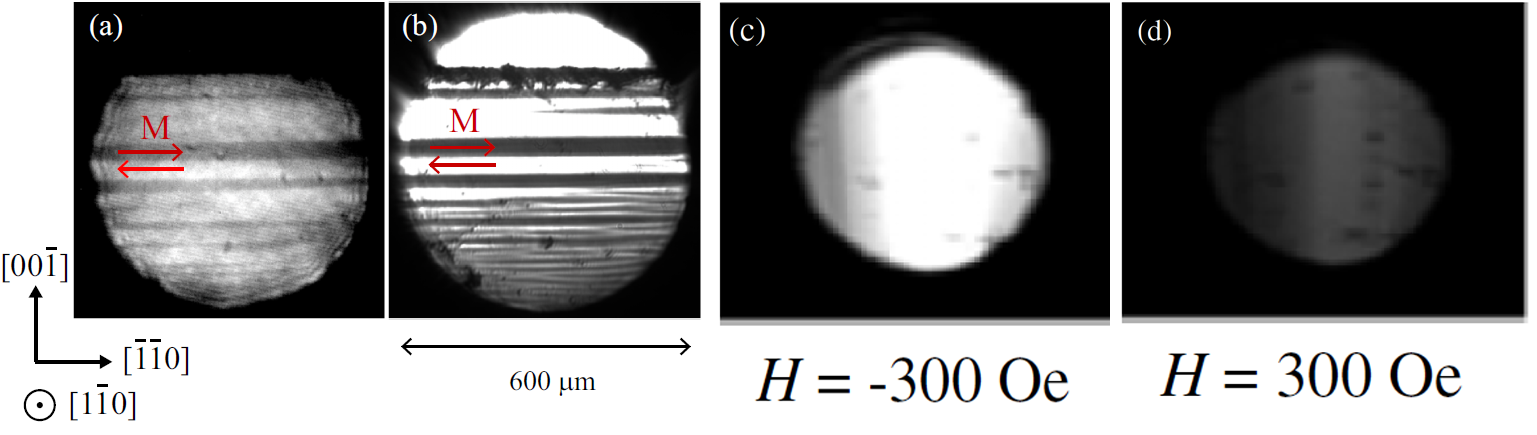
\includegraphics[scale=0.4]{applications}
	}
	\caption{(a), (b) Фотографии магнитных доменов из \autocite{Toyoda2016}, полученные с помощью фотолюминесценции. (c), (d) Фотографии света, прошедшего через пластинку \cbo\, к которой приложили внешнее магнитное поле в -300 и 300~Э~\autocite{Saito2008jpsj}. (a, b) и (c, d) сделаны при одной и той же яркости и контрасте.}\label{fig:applications}
\end{figure}

Можно выделить два подхода в развитии теории магнитоэлектрических эффектов: феноменологический и микроскопический. Феноменологический подход сформулирован в работе Дзялошинского \autocite{Dzyaloshinskii1959}. Этот подход успешно использовался для анализа ряда материалов. Его применение описано во многих обзорах и оригинальных статьях \autocite{Zvezdin2008, Pyatakov2012, Popkov2016}. Микроскопический подход развит слабее и предполагает предварительный анализ энергетических схем уровней и взаимодействий магнитных ионов с обменными и электрическими полями. Как это подчеркивается в обзорах \autocite{Khomskii2009, Moskvin2009, Tokura2014, Shuai2015}, микроскопические механизмы магнитоэлектрической связи еще не вполне выяснены.

%(см. рисунок \cref{fig:applications})

{\aim} данной работы является разработка микроскопической теории статических и динамических магнитоэлектрических эффектов в диэлектрике \cbo\ на основе квантово-механического подхода.

Для~достижения поставленной цели необходимо было решить следующие {\tasks}:
\begin{enumerate}[beginpenalty=10000] % https://tex.stackexchange.com/a/476052/104425
	\item проанализировать и систематизировать имеющиеся на момент написания работы данные по экспериментальному наблюдению и теоретическому описанию магнитоэлектрических эффектов в \cbo;
	\item рассчитать уровни энергии и волновые функции иона меди 3d\(^9\) в кристалле \cbo
	\item оценить параметры взаимодействия электронов меди с электрическим и магнитным полем
	\item попытаться объяснить  имеющиеся экспериментальные данные на основе  единой микроскопической модели 
\end{enumerate}


{\novelty}
\begin{enumerate}[beginpenalty=10000] % https://tex.stackexchange.com/a/476052/104425
	\item Получен эффективный оператор, позволивший объяснить происхождение магнитоэлектрических эффектов в	Cu$_{(1-x)}$Ni$_x$B$_2$O$_4$. Установлено, что они, главным образом, обусловлены ионами \emph{никеля}, а не меди, как предполагалось ранее.  
	\item Построены теоретические диаграммы пространственной асимметрии фотолюминесценции в магнитных полях при различных направлениях  волнового вектора и векторов поляризации.
\end{enumerate}


{\probation}
Основные результаты работы докладывались~на трех конференциях:
\begin{enumerate}[beginpenalty=10000] % https://tex.stackexchange.com/a/476052/104425
	\item \textit{Нурмухаметов, А. Р.} Особенности экситонных зон Френкеля-Давыдова в антиферромагнетиках [Устный доклад] / А.~Р.~Нурмухаметов // Итоговая конференция Института Физики. --- 2021.
	\item \textit{Нурмухаметов, А. Р.} Магнитоэлектрическая связь в Cu\(_{1-x}\)Ni\(_{x}\)B\(_{2}\)O\(_{4}\) [Устный доклад] / А.~Р.~Нурмухаметов // Итоговая конференция Института Физики. --- 2022.
	\item \textit{Нурмухаметов, А. Р.} К теории необратимости в спектрах \cbo\ [Стендовый доклад] / А.~Р.~Нурмухаметов, М.~В.~Еремин // Нанофизика и наноэлектроника. Труды XXVI Международного симпозиума. --- 2022.
\end{enumerate}

Имеются две публикации в журналах:

\begin{enumerate}[beginpenalty=10000] % https://tex.stackexchange.com/a/476052/104425
	\item \textit{Еремин, М. В.} О магнитоэлектрической связи в \ncbo / М.~В.~Еремин, А.~Р.~Нурмухаметов // Письма в ЖЭТФ. --- 2021. --- Т.~114, \textnumero~1. --- С.~31-35. --- URL: \url{https://doi.org/10.31857/S1234567821130073}.
	\item \textit{Нурмухаметов, А. Р.} О магнитоэлектрической связи в \ncbo / А.~Р.~Нурмухаметов, М.~В.~Еремин // ЖЭТФ. --- 2022. --- Т.~162, \textnumero~3. --- С.~1-8. --- URL: \url{https://doi.org/10.31857/S0044451022090000}.
\end{enumerate}


 % Характеристика работы по структуре во введении и в автореферате не отличается (ГОСТ Р 7.0.11, пункты 5.3.1 и 9.2.1), потому её загружаем из одного и того же внешнего файла, предварительно задав форму выделения некоторым параметрам

\textbf{Объем и структура работы.} Диссертация состоит из~введения,
\formbytotal{totalchapter}{глав}{ы}{}{},
заключения и
\formbytotal{totalappendix}{приложен}{ия}{ий}{}.
%% на случай ошибок оставляю исходный кусок на месте, закомментированным
%Полный объём диссертации составляет  \ref*{TotPages}~страницу
%с~\totalfigures{}~рисунками и~\totaltables{}~таблицами. Список литературы
%содержит \total{citenum}~наименований.
%
Полный объём диссертации составляет
\formbytotal{TotPages}{страниц}{у}{ы}{}, включая
\formbytotal{totalcount@figure}{рисун}{ок}{ка}{ков} и
\formbytotal{totalcount@table}{таблиц}{у}{ы}{}.
Список литературы содержит
\formbytotal{citenum}{наименован}{ие}{ия}{ий}.
